Задача узла заключается в формировании выходной импульсной последовательности из входной, выбирая только некоторые, в зависимости от режима, импульсы, с периодом в 22 импульса. Например, в первом режиме (3, 8, 11, 20) на выход подадутся (считая от единицы): 3-й, 8-й, 11-й, 20-й, (3+22)-й, (8+22)-й, (11+22)-й, (20+22)-й и т.д. импульсы.\\
Идея первого варианта узла заключается в следующем. По входному тактовому сигналу работает счётчик, который считает от 0 до 21, циклично. Счётчик формирует 5-разрядное число на выходе. Данные пять разрядов используются, чтобы выбрать один из 22-х выходов дешифратора. Выходы дешифратора объединены в шесть частично пересекающихся групп через элементы ИЛИ, в соответствии со вариантами режимов. Т.е., когда счётчик досчитывает до некоторого числа n (т.е. когда на вход приходит (n+1)-й импульс), элементы ИЛИ, в которые входит данное число, выдают логическую единицу, все остальные - логический ноль. Таким образом осуществляется фильтрация входного тактового сигнала в соответствии со всеми режимами, формируется шесть импульсных последовательностей. При помощи мультиплексора, по номеру режима, осуществляется коммутация одной из этих последовательностей на выход. Функциональная схема данного узла представлена на рис. \ref{fig:firstnode}.
\begin{figure}
  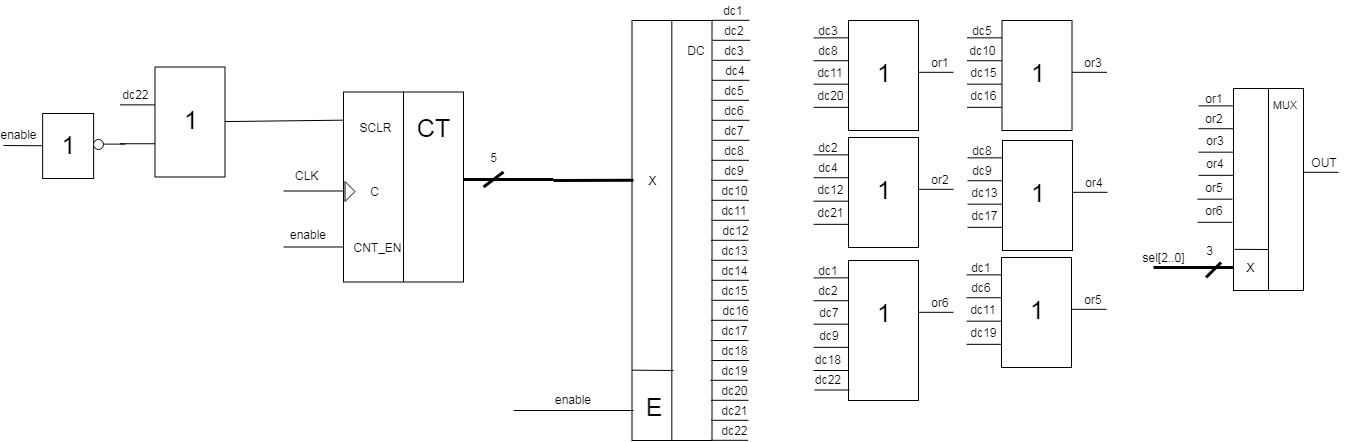
\includegraphics[scale=0.35]{./first-node.png}
  \caption{Функциональная схема многорежимного формирователя импульсной последовательности. Вариант 1.}
  \label{fig:firstnode}
\end{figure}